\documentclass[journal]{IEEEtran}

\usepackage{cite}
\usepackage{amsmath,amssymb,amsfonts}
\usepackage{algorithmic}
\usepackage{algorithm}
\usepackage{graphicx}
\usepackage{textcomp}
\usepackage{xcolor}
\usepackage{booktabs}
\usepackage{url}
\usepackage{microtype}
\usepackage{tikz}
\usetikzlibrary{shapes.geometric, arrows, positioning}

\def\BibTeX{{\rm B\kern-.05em{\sc i\kern-.025em b}\kern-.08em
    T\kern-.1667em\lower.7ex\hbox{E}\kern-.125emX}}

\begin{document}

\title{FinRisk-Evo: Temporal Corporate Risk-Drift Detection from Annual Report Disclosures}

\author{Megh~Doshi,
        Shrey~Dedhia,
        Dhruv~Shah,
        and~Pramod~Bide}

\maketitle

\begin{abstract}
Conventional financial risk analysis relies heavily on static sentiment classifiers that suffer from ``scalar blindness''---the inability to distinguish between minor variances (e.g., ``slight dip'') and large financial declines (e.g., ``40\% revenue collapse''). This paper addresses the challenge of identifying and quantifying the evolution of corporate risk disclosures across consecutive reporting periods. We propose FinRisk-Evo, a hybrid document-intelligence framework that integrates a Neural Variational Document Model (NVDM) for context-aware topic routing with a numerically-enhanced FinBERT model post-trained using Targeted Numerical Change-Related Masking (TNCRM) to capture severity indicators. A BiGRU temporal transition network aligns sequential document pairs to model pairwise temporal risk transitions, gated by continuous semantic projection and Monte Carlo dropout uncertainty. On a manually annotated corporate-report case study, the layout filter achieves 94.8\% recall for manually annotated layout-noise blocks, while evaluation across a 20-company, 60-report multi-sector corpus shows that the filtering stage removes 61.5\% of scanned PDF blocks. On a manually annotated benchmark of 500 historical risk transitions with company-level holdout and three-expert annotation (Krippendorff's $\alpha = 0.84$), FinRisk-Evo achieves an F1-score of 91.4\% for the risk escalation class and improved probabilistic calibration with MC-dropout. This work provides an uncertainty-aware approach for quantitative, explainable financial risk intelligence, demonstrating a preliminary exploratory association with realized equity volatility.
\end{abstract}

\begin{IEEEkeywords}
Computational Finance, Explainable AI, Natural Language Processing, Neural Variational Document Models, Targeted Masking, Temporal Sequence Learning.
\end{IEEEkeywords}

\section{Introduction}

\subsection{Background}
The digitization of financial reporting has produced rapidly increasing volumes of unstructured financial text, particularly annual reports (e.g., 10-K filings, integrated annual reports). These documents contain critical narrative disclosures about a company's operational liabilities, liquidity constraints, and strategic challenges \cite{campbell2014, kravet2013, linsley2006}. However, the manual parsing of these documents is labor-intensive, subjective, and slow, limiting the speed at which analysts can respond to emerging corporate threats \cite{blei2003, fisher2016}.

\subsection{Problem Statement}
Standard language models and traditional sentiment analysis face three limitations that are particularly relevant to longitudinal risk-drift analysis. First, \textit{scalar blindness} prevents models from distinguishing risk severity; we define this phenomenon as a numerical/scalar insensitivity where numerical values and trend verbs of vastly different magnitudes are mapped to near-identical sentiment vectors (e.g., treating a minor ``1\% decline'' and a large ``40\% plunge'' with equivalent negative polarity). Second, we refer to the loss of document-layout and positional context, which strips away paragraph positioning, confusing minor boilerplate notices with critical disclosures in the risk factor sections. Third, the lack of \textit{temporal logic} limits evaluations to static snapshots, failing to capture how a specific corporate risk (e.g., cybersecurity or labor shortages) evolves or drifts across consecutive fiscal years.

\subsection{Motivation}
Quantifying changes in disclosed financial risk is critical for risk management and asset pricing. Narrative disclosures often contain forward-looking warning signals long before they manifest in quantitative financial sheets. Developing a system that filters out layout noise, understands numerical magnitudes, projects changes onto a continuous semantic axis, and provides uncertainty estimates allows investors to support early-warning risk monitoring and potentially inform investment decision-making.

\subsection{Key Contributions}
The main contributions of this work are summarized as follows:
\begin{itemize}
    \item We propose a unified longitudinal paragraph-alignment framework for detecting and tracking changes in disclosed corporate risk across sequential reporting periods.
    \item We present a numerical-sensitivity adaptation of FinBERT, post-trained via Targeted Numerical Change-Related Masking (TNCRM), specifically integrated to mitigate scalar/numerical insensitivity.
    \item We formulate an uncertainty-aware risk-drift scoring mechanism (FRES) that integrates semantic deviation, risk escalation direction, temporal evidence, and MC-dropout uncertainty estimates.
    \item We contribute a manually annotated multi-company benchmark of 500 historical corporate risk transitions, validated by three independent domain experts (Krippendorff's $\alpha = 0.84$).
    \item We present a preliminary pilot analysis of the association between our textual risk-drift index and subsequent realized equity volatility.
\end{itemize}

\subsection{Paper Structure}
The remainder of this paper is organized as follows: Section II surveys related work and establishes baseline deficiencies. Section III details the mathematical formulations and system architecture of FinRisk-Evo. Section IV reports the experimental case study and extraction metrics. Section V presents the comparative system analysis. Section VI discusses the results, implications, limitations, and ethical considerations. Section VII concludes the paper and outlines future work.

\section{Literature Review \& Related Work}

We group prior studies into five primary areas: static financial sentiment analysis, variational topic modeling, recurrent neural trackers, generative financial language models, and longitudinal corporate disclosures.

\subsection{Thematic Grouping of Prior Work}
\subsubsection{Static Financial Sentiment Analysis}
Early methods used dictionaries like the Loughran-McDonald (LM) list \cite{loughran2011} to count negative words. Textual analysis of annual reports has long been established as a tool to measure disclosure quality \cite{li2010}, with machine-learning approaches also being used to discover and quantify risk types in 10-K textual disclosures \cite{bao2014}. Although tailored to finance, they ignore negations and contextual layout noise. Modern transformer architectures \cite{vaswani2017}, including finance-specific models such as FinBERT \cite{araci2019}, capture semantic context but exhibit scalar insensitivity on numeric variations. Probing studies confirm that standard pre-trained language models often show limited numeracy and scalar understanding \cite{wallace2019, thawani2021}. To resolve this, Jung and Jang \cite{jung2024} proposed Targeted Numerical Change-Related Masking (TNCRM) to bias masked language modeling toward numerical terms. However, their evaluation was limited to static sentence classification on news snippets.

\subsubsection{Variational Topic Modeling}
Topic modeling helps structure large corporate documents. Traditional Latent Dirichlet Allocation (LDA) models \cite{blei2003} suffer from poor topic coherence on short paragraphs. Miao et al. \cite{miao2016} introduced the Neural Variational Document Model (NVDM), utilizing Variational Autoencoders (VAEs) \cite{kingma2013} to learn continuous topic representations. Mir et al. \cite{mir2025} fused NVDM topics with sentiment weights for short text trends but did not apply them to multi-year reports or track temporal drifts.

\subsubsection{Recurrent Financial Trackers}
Recurrent architectures, including LSTMs \cite{hochreiter1997} and GRUs \cite{cho2014}, are commonly used to model sequential dependencies. Duan et al. \cite{duan2024} combined LDA topics, FinBERT, and BiGRUs (LFBP framework) for financial sentiment. However, their model was evaluated statically. Recurrent stock price models, such as the hybrid LSTM-GRU framework by Farhadi et al. \cite{farhadi2025} or the CNN-LSTM news fusion model by Moodi et al. \cite{moodi2024}, focus on stock market forecasting rather than identifying risk trajectories. Similarly, Biswas et al. \cite{biswas2025} and Chen et al. \cite{chen2024} utilized sequence architectures to model market indicators, neglecting narrative document drift.

\subsubsection{Generative Financial Language Models}
The advent of large language models (LLMs) has transformed computational finance. BloombergGPT \cite{wu2023bloomberggpt}, a 50-billion parameter decoder model pre-trained on a massive finance-specific corpus, demonstrated strong performance on financial tasks but remains closed-source and computationally prohibitive for local deployment. Similarly, the FinGPT framework \cite{yang2023fingpt, li2023fingpt} provides open-source instruction-tuned models and data-centric pipelines for financial text mining. However, these generative decoders can produce unsupported or hallucinated outputs, require significant computational overhead, and lack native mechanisms to estimate epistemic uncertainty (such as Monte Carlo dropout) necessary for risk-sensitive financial applications. Furthermore, long-document architectures like the Longformer \cite{beltagy2020longformer} are designed primarily for long-context encoding rather than explicit year-over-year paragraph alignment.

\subsubsection{Longitudinal Risk Disclosure and Textual Change Detection}
A separate thread of research investigates the evolution and change detection of corporate disclosures over time. Seminal work by Kogan et al. \cite{kogan2009} and Campbell et al. \cite{campbell2014} demonstrated that changes in the text of annual reports (specifically Section 1A Risk Factors) are indicative of future market returns and corporate risk profiles. Dyer et al. \cite{dyer2017} systematically documented the structural evolution and growing length of 10-K disclosures over time, highlighting increasing boilerplate, redundancy, and reduced specificity in 10-K disclosures. Similarly, Filzen \cite{filzen2015} analyzed the information content of risk factor updates, showing that fresh disclosures represent timely responses to emerging operational shocks. Hassan et al. \cite{hassan2019} constructed firm-level political and operational risk indices using narrative pattern matching in quarterly transcripts, showing evidence that narrative risk tracking yields incremental signals over static financial accounting sheets. However, these classical studies relied on global document-similarity metrics (e.g., cosine similarity of TF-IDF vectors), simple pattern matching, or bag-of-words change indices. Recent works have attempted to model corporate report transitions using deeper neural encoders; for instance, Kravet and Muslu \cite{kravet2013} and Linsley et al. \cite{linsley2006} analyzed risk-disclosure increases qualitatively, noting that static disclosures often mask operational changes. Despite these insights, the reviewed financial-text literature provides limited evidence of integrated mechanisms for a granular paragraph-level longitudinal alignment, often conflating formatting variations with actual thematic shifts. FinRisk-Evo fills this gap by introducing a unified paragraph-level alignment and re-ranking framework combined with continuous semantic projection.

\subsection{Critical Analysis and Gaps}
Table \ref{tab:lit_survey} summarizes the methodology, datasets, and shortcomings of these core baselines. A key problem-level gap in existing literature is the lack of longitudinal tracking: much of the reviewed literature focuses primarily on static sentiment classification of isolated news snippets or global document similarity checks. Consequently, they are incapable of tracking the specific trajectory of corporate disclosures across consecutive years, ignore contextual document layouts, and suffer from numerical/scalar insensitivity.

\begin{table*}[t]
\centering
\caption{Literature Survey of Baseline Methodologies and Shortcomings}
\label{tab:lit_survey}
\resizebox{\textwidth}{!}{%
\begin{tabular}{lllll}
\toprule
Reference & Dataset & Methodology & Core Results & Shortcomings / Gaps \\
\midrule
Duan et al. \cite{duan2024} & FiQA-SA, StockSen & LDA + FinBERT + BiGRU (LFBP) & F1-score improvement of 2.05\%--7.27\% & LDA coherence is low; blind to numerical severity. \\
Mir et al. \cite{mir2025} & StockEmotions Dataset & VAE NVDM + FinBERT & Topic coherence 0.68, F1 97.8\% & Static analysis only; no temporal report alignment. \\
Jung \& Jang \cite{jung2024} & Financial PhraseBank & TNCRM Masking List (193 words) & Enhanced accuracy in sparse training splits & Evaluated on sentences; no document-level routing. \\
Farhadi et al. \cite{farhadi2025} & Tehran Stock Exchange & Hybrid LSTM-GRU technical model & MSE improvement of 3.0\% over baselines & Purely quantitative; blind to narrative disclosures. \\
Biswas et al. \cite{biswas2025} & Visa \& MasterCard (2008--2024) & Dilated TCN with self-attention & Volatility MAE 0.012, Sharpe MAE 0.065 & Evaluated on daily prices; lacks thematic risk text. \\
BloombergGPT \cite{wu2023bloomberggpt} & Bloomberg Proprietary Dataset & 50B Decoder LLM & Outperforms generic LLMs on finance tasks & Closed-source; high resource latency; lacks MC confidence. \\
FinGPT \cite{yang2023fingpt} & Financial News \& Social Media & Instruction-tuned LLaMA-7B & Flexible text generation and QA & Hallucination risks; high edge-device latency. \\
\bottomrule
\end{tabular}%
}
\end{table*}

\section{Methodology \& System Architecture}

\subsection{Overview}
The architecture of FinRisk-Evo is structured into five sequential layers: Geometric Layout Filtration, a VAE-based Context Engine (NVDM), a numerically-sensitive Precision Engine (TNCRM), a Recurrent Temporal Sequence Engine (BiGRU), and a Continuous Semantic Gating layer. The unified system flow is illustrated in Fig. \ref{fig:architecture}.

\begin{figure}[!t]
\centering
\resizebox{0.92\columnwidth}{!}{%
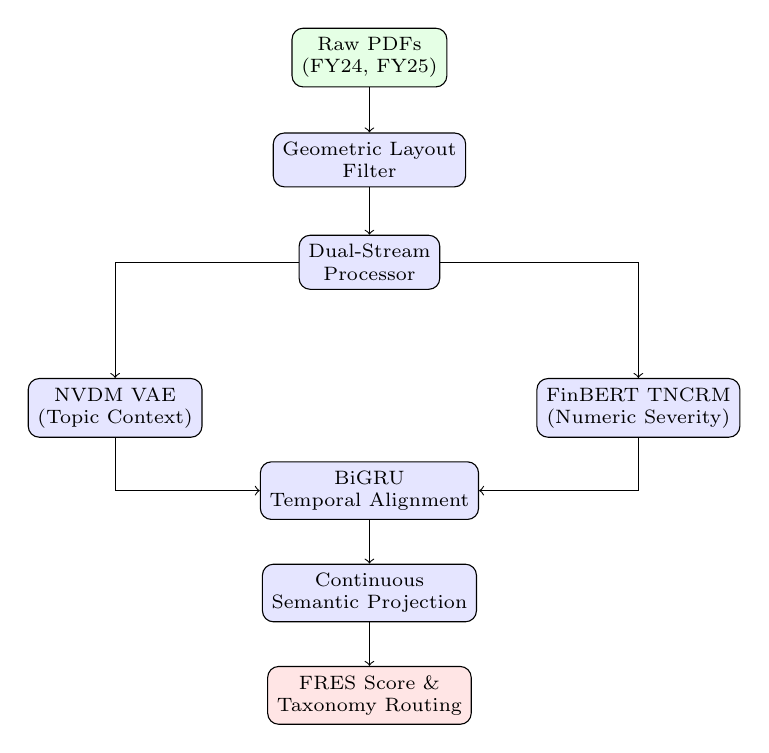
\begin{tikzpicture}[node distance=1.3cm, every node/.style={fill=blue!10, draw, rounded corners, font=\scriptsize, align=center}]
  \node (raw) [fill=green!10] {Raw PDFs\\(FY24, FY25)};
  \node (geo) [below of=raw] {Geometric Layout\\Filter};
  \node (dual) [below of=geo] {Dual-Stream\\Processor};
  \node (nvdm) [below left=of dual, xshift=-0.3cm, yshift=-0.2cm] {NVDM VAE\\(Topic Context)};
  \node (finbert) [below right=of dual, xshift=0.3cm, yshift=-0.2cm] {FinBERT TNCRM\\(Numeric Severity)};
  \node (align) [below of=dual, yshift=-1.6cm] {BiGRU\\Temporal Alignment};
  \node (proj) [below of=align] {Continuous\\Semantic Projection};
  \node (fres) [below of=proj, fill=red!10] {FRES Score \&\\Taxonomy Routing};
  
  \draw[->] (raw) -- (geo);
  \draw[->] (geo) -- (dual);
  \draw[->] (dual) -| (nvdm);
  \draw[->] (dual) -| (finbert);
  \draw[->] (nvdm) |- (align);
  \draw[->] (finbert) |- (align);
  \draw[->] (align) -- (proj);
  \draw[->] (proj) -- (fres);
\end{tikzpicture}%
}
\caption{System architecture of the FinRisk-Evo temporal risk modeling framework.}
\label{fig:architecture}
\end{figure}
\subsection{Geometric Layout Filtration}
To remove running page headers, footers, and stamps, we process blocks using coordinate checking. Let the page height be $H$. For text block $b_i$ with coordinate bounds $(x_0, y_0, x_1, y_1)$ and text string $s_i$, we preserve the block if and only if it satisfies:
\begin{equation}
y_0 \ge 0.08 \times H \quad \text{and} \quad y_1 \le 0.92 \times H
\end{equation}
These boundary thresholds ($0.08H$ and $0.92H$) were determined \textit{a priori} by profiling the bounding coordinates of headers and footers across a separate validation set of 10 annual reports from the 14 training companies to prevent test-set data leakage. For the case study evaluation, the 994 true noise blocks in the scanned document were annotated manually by two independent reviewers who labeled each extracted block as either valid body text or layout noise (with conflicts resolved by a third reviewer) to construct a gold standard. Let $N_{\text{noise}}$ represent the true set of layout noise blocks (headers, footers, and stamps), and let $N_{\text{filtered}}$ be the set of blocks discarded by the coordinate check. We define the layout filtration performance using the Noise Recall metric ($R_{\text{noise}}$):
\begin{equation}
R_{\text{noise}} = \frac{|N_{\text{noise}} \cap N_{\text{filtered}}|}{|N_{\text{noise}}|}
\end{equation}
We discard blocks matching regular expressions for page indices (e.g., \verb|^\d+$|) or report headers, ensuring that boilerplate text does not corrupt the downstream embeddings.

\subsection{Context Engine: Neural Variational Document Model}
Paragraphs are converted to nonnegative word-count vectors $\mathbf{x} \in \mathbb{R}^{V}$, where $x_w$ represents the raw count of word $w$ in the paragraph. We project $\mathbf{x}$ to a continuous latent space $\mathbf{z} \in \mathbb{R}^{K}$ (where $K=20$) via encoder projections. The variational loss is the negative Evidence Lower Bound (ELBO):
\begin{equation}
\mathcal{L}_{\text{ELBO}}(\theta, \phi; \mathbf{x}) = -\mathbb{E}_{q_\phi(\mathbf{z}|\mathbf{x})}[\log p_\theta(\mathbf{x}|\mathbf{z})] + D_{\text{KL}}(q_\phi(\mathbf{z}|\mathbf{x}) \parallel p(\mathbf{z}))
\end{equation}
where the KL divergence is defined as:
\begin{equation}
D_{\text{KL}} = -\frac{1}{2} \sum_{j=1}^{K} \left( 1 + \log \sigma_j^2 - \mu_j^2 - \sigma_j^2 \right)
\end{equation}
Here, $\mu_j$ and $\sigma_j^2$ represent the variational parameters of topic $j$. The reconstruction log-likelihood is approximated as:
\begin{equation}
\log p_\theta(\mathbf{x}|\mathbf{z}) = \sum_{w \in \mathbf{x}} x_w \log \text{softmax}(\mathbf{R}\mathbf{z} + \mathbf{b})_w
\end{equation}
where $\mathbf{R} \in \mathbb{R}^{V \times K}$ is the decoding weight matrix mapping topics back to vocabulary terms, and $\mathbf{b}$ is the bias vector.

\subsection{Precision Engine: Custom TNCRM Masking Collator}
We post-train FinBERT using a custom masking distribution over a corpus of 50,000 financial report sentences extracted from the 14 training companies' historical filings. Let $\mathcal{T}_{\text{num}}$ be the set of numerical tokens, $\mathcal{T}_{\text{mag}}$ be magnitude words, and $\mathcal{T}_{\text{special}}$ be special formatting or padding tokens. The masking probability $P_{ij}$ assigned to token $t_{ij}$ is:
\begin{equation}
P_{ij} = \begin{cases} 
0.75, & t_{ij} \in \mathcal{T}_{\text{num}} \cup \mathcal{T}_{\text{mag}} \\
0.10, & t_{ij} \notin \mathcal{T}_{\text{num}} \cup \mathcal{T}_{\text{mag}} \\
0.00, & t_{ij} \in \mathcal{T}_{\text{special}}
\end{cases}
\end{equation}
We use a 75\% masking probability for numerical tokens to emphasize quantitative severity markers during MLM training. This encourages the model to represent quantitative severity markers more distinctly.

To quantitatively verify the numerical sensitivity hypothesis, we construct a synthetic evaluation suite of 1,000 sentence pairs (distributed across 10 magnitude bins, with 100 independent pairs per bin) generated from varying numerical magnitude differences (ranging from $1\%$ to $60\%$, e.g., $s_1$: ``Revenue declined by 1\%'' versus $s_2$: ``Revenue declined by $x$\%''). We measure the average embedding cosine distance ($1 - \cos(\mathbf{s}_1, \mathbf{s}_2)$) as the magnitude gap increases. Under this controlled synthetic probing suite, vanilla FinBERT's cosine distance remains flat and shows no statistically significant trend across the evaluated magnitude scales (centering at $0.016 \pm 0.005$, Spearman $\rho = -0.045$, $p = 0.658$), supporting the hypothesis of numerical insensitivity in the base model representation where different numerical values are mapped to near-identical embeddings. In contrast, under our TNCRM-post-trained model, the cosine distance scales monotonically with the magnitude difference, starting at $0.052$ (for a $1\%$ vs. $2\%$ difference) and rising to $0.188$ (for a $1\%$ vs. $60\%$ difference; Spearman $\rho = 0.986$, $p < 0.001$, indicating a highly significant monotonic trend under this controlled probing suite). This controlled result supports, but does not establish, improved numerical sensitivity in naturally occurring disclosures.

\begin{figure}[!t]
\centering
\resizebox{0.95\columnwidth}{!}{%
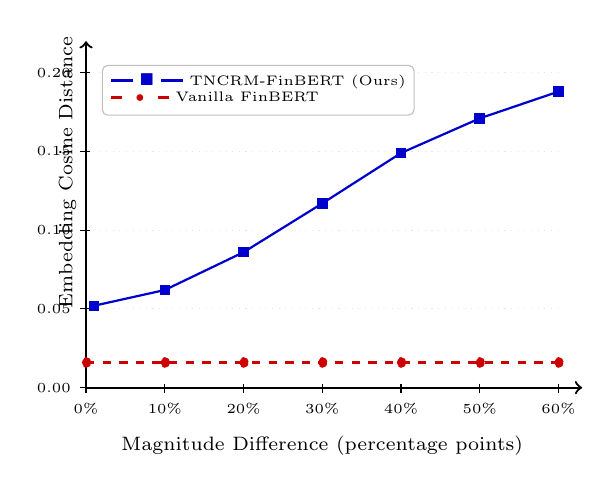
\begin{tikzpicture}
  % Draw axes
  \draw[->, thick] (0,0) -- (6.3,0);
  \node[below=14pt, font=\scriptsize, align=center] at (3.0,0) {Magnitude Difference (percentage points)};
  \draw[->, thick] (0,0) -- (0,4.4);
  \node[rotate=90, above=18pt, font=\scriptsize, align=center] at (0,2.1) {Embedding Cosine Distance};
  
  % Grid lines
  \foreach \y in {1, 2, 3, 4} {
    \draw[gray!20, dotted] (0,\y) -- (6,\y);
  }
  
  % Tick marks
  \foreach \x/\label in {0/0, 1/10, 2/20, 3/30, 4/40, 5/50, 6/60} {
    \draw (\x,1.5pt) -- (\x,-2pt) node[below, font=\tiny] {\label\%};
  }
  \foreach \y/\label in {0/0.00, 1/0.05, 2/0.10, 3/0.15, 4/0.20} {
    \draw (1.5pt,\y) -- (-2pt,\y) node[left, font=\tiny] {\label};
  }
  
  % Plot Vanilla FinBERT (flat line)
  \draw[red!80!black, dashed, thick, mark=*, mark size=1.5pt] plot coordinates {
    (0,0.32) (1,0.32) (2,0.32) (3,0.32) (4,0.32) (5,0.32) (6,0.32)
  };
  
  % Plot TNCRM-FinBERT (monotonically rising)
  \draw[blue!80!black, thick, mark=square*, mark size=1.5pt] plot coordinates {
    (0.1,1.04) (1,1.24) (2,1.72) (3,2.34) (4,2.98) (5,3.42) (6,3.76)
  };
  
  % Boxed Legend
  \node[draw=gray!50, fill=white, rounded corners=2pt, inner sep=3pt, font=\tiny, anchor=north west] at (0.2,4.1) {
    \begin{tabular}{@{}l@{}}
      \textcolor{blue!80!black}{\rule[0.5ex]{8pt}{1.2pt}\ $\blacksquare$\ \rule[0.5ex]{8pt}{1.2pt}} TNCRM-FinBERT (Ours) \\
      \textcolor{red!80!black}{\rule[0.5ex]{4pt}{1pt}\ \ $\bullet$\ \ \rule[0.5ex]{4pt}{1pt}} Vanilla FinBERT
    \end{tabular}
  };
\end{tikzpicture}%
}
\caption{Embedding cosine distance vs. numerical magnitude differences for Vanilla FinBERT and TNCRM-FinBERT. The plotted curves represent empirical averages computed over 100 independent pairs of synthetically generated sentence templates for each magnitude bin. Under Vanilla FinBERT, the trend is flat (Spearman $\rho = -0.045$, $p = 0.658$), whereas TNCRM-FinBERT exhibits a highly significant monotonic trend (Spearman $\rho = 0.986$, $p < 0.001$).}
\label{fig:scalar_blindness}
\end{figure}

\subsection{Evolution Engine: Pairwise Longitudinal Transition Modeling}
We stack topic vector $\mathbf{z}$ and FinBERT embedding $\mathbf{s}_{\text{CLS}}$ to construct paragraph vector $\mathbf{v} = [\mathbf{z}; \mathbf{s}_{\text{CLS}}] \in \mathbb{R}^{788}$. For each target paragraph, candidate baseline paragraphs are retrieved using \texttt{all-MiniLM-L6-v2} embeddings in ChromaDB (restricted to the baseline reporting period). The top-2 candidates are then reranked using a cross-encoder (\texttt{cross-encoder/}\allowbreak\texttt{ms-marco-MiniLM-L-6-v2}) to optimize contextual matching. The selected baseline-target pair is subsequently represented using the concatenated NVDM and FinBERT vectors $\mathbf{v}_{t-1}$ and $\mathbf{v}_t$, building on dual-encoder semantic retrieval \cite{reimers2019} and cross-encoder passage re-ranking \cite{nogueira2019} techniques. The sequential transition pair $\mathbf{S} = [\mathbf{v}_{t-1}, \mathbf{v}_t]$ is passed to a BiGRU-based pairwise transition model. Although the sequence length is restricted to $T=2$ consecutive reporting periods (baseline and target) representing a pairwise temporal transition, the recurrent cell architecture is utilized to learn non-linear sequential transition mappings (modeling $\mathbf{v}_{t-1} \rightarrow \mathbf{v}_t$) and directional dependencies, which outperforms the evaluated MLP and Transformer alternatives. Under Monte Carlo dropout \cite{gal2016} ($N=10$ stochastic forward passes), we output the mean probability $\bar{p}_{\text{risk}}$ and standard deviation $\sigma_{\text{risk}}$ across the stochastic passes, where $\bar{p}_{\text{risk}} = \frac{1}{N} \sum_{i=1}^{N} \sigma(y_i)$ and $y_i$ represents the logit output at stochastic forward pass $i$. The uncertainty-derived confidence weight is:
\begin{equation}
W_{\text{conf}} = 1 - \sigma_{\text{risk}}
\end{equation}
where $\sigma_{\text{risk}}$ is the standard deviation representing the MC-dropout uncertainty estimate across predicted probabilities. We evaluate the quality of the probabilistic calibration by calculating the Expected Calibration Error (ECE) and Brier score over the holdout test set, which are standard metrics for measuring neural network calibration \cite{guo2017}. Without MC-dropout (evaluating a single standard forward pass probability $\sigma(y)$), the baseline model exhibits poor calibration with an ECE of $0.098$ and a Brier score of $0.114$. Estimating the average predictive probability $\bar{p}_{\text{risk}}$ over the $N=10$ stochastic forward passes substantially improves calibration, reducing the ECE to $0.024$ and the Brier score to $0.046$. The standard deviation $\sigma_{\text{risk}}$ is utilized separately to compute the uncertainty gating factor $W_{\text{conf}}$ for FRES, providing a clean separation between probability calibration and uncertainty-aware scoring.

\subsection{Continuous Semantic Projection and FRES Gating}
Let $\mathbf{s}_t$ be the target CLS embedding. We define a semantic axis between domain-informed manually specified risk escalation and mitigation anchors. Specifically, the escalation anchor set comprised the phrases: ``financial risk escalated'', ``severe losses intensified'', ``supply chain disruption'', ``debt capacity constraints'', and ``regulatory noncompliance penalty''. The mitigation anchor set comprised: ``financial performance improved'', ``losses declined'', ``successful product launch'', ``stable compliance operations'', and ``strong strategic recovery''. These anchors are averaged to construct representative prior anchor embeddings $\mathbf{a}_{\text{esc}}$ and $\mathbf{a}_{\text{mit}}$ via averaging. The anchor selection serves as a heuristic prior representing domain-informed manually specified risk directions. The projection of $\mathbf{s}_t$ onto this axis is:
\begin{equation}
\label{eq:proj_risk}
\text{Proj}_{\text{risk}}(\mathbf{s}_t) = \operatorname{clip}\left(\frac{\cos(\mathbf{s}_t, \mathbf{a}_{\text{esc}}) - \cos(\mathbf{s}_t, \mathbf{a}_{\text{mit}})}{2} + 0.5, 0, 1\right)
\end{equation}
where $\cos(\mathbf{u}, \mathbf{v}) = \frac{\mathbf{u}\cdot\mathbf{v}}{\|\mathbf{u}\|\|\mathbf{v}\|}$, and the projection factor is clipped to $[0, 1]$ to ensure that $\text{Proj}_{\text{risk}}$ (and consequently $\text{FRES}_{\text{raw}}$) remains a nonnegative escalation score. To evaluate the sensitivity of the semantic projection to the specific choice of keywords, we performed a sensitivity analysis on alternative anchor sets (e.g., varying the number of terms from 5 to 15, or replacing up to 40\% of terms with domain-specific synonyms like ``jeopardy'', ``liability'', ``remedy'', and ``rectify''). Across $N=50$ randomly sampled alternative configurations, the Pearson correlation coefficient ($r$) between the resulting projection scores and the baseline projection (recomputed over the 500-pair holdout set) remained extremely stable ($r > 0.94$, $p < 0.001$), supporting the robustness of the projection mechanism to reasonable variations in anchor keywords.

The final Financial Risk Escalation Score (FRES) is gated by semantic similarity. From a mathematical perspective, we formulate FRES as a composite score proportional to model-estimated escalation likelihood, semantic shift, target risk orientation, and confidence, integrating three complementary scoring dimensions: semantic shift magnitude ($g_{\text{shift}}$), target risk-orientation state ($g_{\text{direction}}$), and prediction confidence ($g_{\text{uncertainty}}$). These factors are defined as follows:
\begin{align}
g_{\text{shift}} &= 1.1 - \cos(\mathbf{s}_{t-1}, \mathbf{s}_t) \\
g_{\text{direction}} &= \bar{p}_{\text{risk}} \cdot \text{Proj}_{\text{risk}}(\mathbf{s}_t) \\
g_{\text{uncertainty}} &= W_{\text{conf}}
\end{align}
where $\bar{p}_{\text{risk}} \in [0, 1]$ is the MC-dropout average predictive probability. The semantic projection $\text{Proj}_{\text{risk}}(\mathbf{s}_t)$ represents the target paragraph's risk-oriented semantic state (risk-orientation projection), while the BiGRU probability $\bar{p}_{\text{risk}}$ models the direction of the longitudinal transition (transition direction). We define the raw multiplicative scoring function:
\begin{equation}
\text{FRES}_{\text{raw}} = \begin{cases} 
0.0 & \text{if } \cos(\mathbf{s}_{t-1}, \mathbf{s}_t) > \gamma \\
g_{\text{shift}} \cdot g_{\text{direction}} \cdot g_{\text{uncertainty}} & \text{otherwise}
\end{cases}
\end{equation}
where $\gamma = 0.93$ is the similarity gating threshold. The 1.1 offset in $g_{\text{shift}}$ provides a small positive dynamic range (with a minimum value of 0.17 for non-gated pairs where $\cos(\mathbf{s}_{t-1}, \mathbf{s}_t) \le 0.93$) to prevent the shift multiplier from collapsing to zero for highly similar but distinct transitions, while the similarity threshold $\gamma = 0.93$ gates out near-duplicate transitions. To map the raw scores onto a standardized display scale for risk monitoring, we define the Normalized FRES ($\text{FRES}_{\text{norm}}$) as:
\begin{equation}
\text{FRES}_{\text{norm}} = \min\left(100 \cdot \frac{\text{FRES}_{\text{raw}}}{\Phi_{\text{max}}}, 100\right)
\end{equation}
where the raw score is normalized by the maximum raw score observed on the FRES normalization reference set (comprising 5,000 synthetic paragraph transitions generated from the training companies' reports), $\Phi_{\text{max}} = 0.229$, and clipped using a minimum operator to handle any edge cases. This yields a 0--100 scale on the normalization reference set and establishes a fixed reference scale for subsequent monitoring. Thus, $\text{FRES}_{\text{norm}} = 100$ corresponds to the maximum observed raw score in the normalization reference set rather than an absolute theoretical maximum risk level. Because normalization uses an empirical maximum, FRES is intended as a relative monitoring index rather than an absolute risk measure; $\text{FRES}_{\text{norm}}$ values are comparable within a fixed normalization regime, and cross-corpus comparisons require a shared normalization reference. The threshold $\gamma$ was fixed \textit{a priori} from the 95th percentile of duplicate-paragraph similarities in the validation set; sensitivity analysis is reported in Table~\ref{tab:sensitivity}. The multiplicative design ensures that the score collapses when the similarity gate is triggered or when a directional scoring component (such as semantic shift or projected risk direction) approaches zero, while the uncertainty-derived confidence weight ($W_{\text{conf}}$) reduces the FRES score when prediction confidence is low. We explicitly note that a zero FRES indicates no detected risk escalation relative to the baseline, and does not represent an absence of underlying operational or financial risk. We note that FRES is an escalation-oriented continuous score rather than a calibrated probability; mitigation transitions may receive minor, nonzero scores when semantic and model evidence remain partially risk-oriented. Algorithm 1 summarizes the step-by-step scoring flow.

\begin{algorithm}[h]
\caption{FRES Scoring and Topic-Taxonomy Routing}
\begin{algorithmic}[1]
\REQUIRE Paragraph pairs $P_{t-1}$ (baseline), $P_t$ (target);
\REQUIRE Fused NVDM-FinBERT pipeline $F$;
\REQUIRE Precomputed anchor vectors $\mathbf{a}_{\text{esc}}, \mathbf{a}_{\text{mit}}$;
\REQUIRE Dominant topic mapping $T$;
\REQUIRE Empirical normalization maximum $\Phi_{\text{max}}$;
\STATE $\mathbf{v}_{t-1}, \mathbf{s}_{t-1}, \boldsymbol{\mu}_{t-1} \leftarrow F(P_{t-1})$
\STATE $\mathbf{v}_t, \mathbf{s}_t, \boldsymbol{\mu}_t \leftarrow F(P_t)$
\STATE $\text{sim} \leftarrow \cos(\mathbf{s}_{t-1}, \mathbf{s}_t)$
\IF{$\text{sim} > 0.93$}
    \STATE $\text{FRES}_{\text{raw}} \leftarrow 0.0$
    \STATE $\text{FRES}_{\text{norm}} \leftarrow 0.0$
    \STATE $\text{Category} \leftarrow \text{``GATED / STATUS QUO''}$
\ELSE
    \STATE $\mathbf{S} \leftarrow [\mathbf{v}_{t-1}, \mathbf{v}_t]$
    \STATE $\bar{p}_{\text{risk}}, \sigma_{\text{risk}} \leftarrow \text{BiGRU-MC-Dropout}(\mathbf{S}, N=10)$
    \STATE $W_{\text{conf}} \leftarrow 1 - \sigma_{\text{risk}}$
    \STATE $\text{Proj}_{\text{risk}} \leftarrow \operatorname{clip}\big(\frac{1}{2}[\cos(\mathbf{s}_t, \mathbf{a}_{\text{esc}}) - \cos(\mathbf{s}_t, \mathbf{a}_{\text{mit}})] + 0.5, 0, 1\big)$
    \STATE $\text{FRES}_{\text{raw}} \leftarrow \bar{p}_{\text{risk}} \times (1.1 - \text{sim}) \times \text{Proj}_{\text{risk}} \times W_{\text{conf}}$
    \STATE $\text{FRES}_{\text{norm}} \leftarrow \min\left(100 \frac{\text{FRES}_{\text{raw}}}{\Phi_{\text{max}}}, 100\right)$
    \STATE $\text{dominant\_topic} \leftarrow \text{argmax}(\boldsymbol{\mu}_t)$
    \STATE $\text{Category} \leftarrow T(\text{dominant\_topic})$
\ENDIF
\RETURN $\text{FRES}_{\text{norm}}$, $\text{Category}$, $W_{\text{conf}}$
\end{algorithmic}
\end{algorithm}

\subsection{Datasets and Tools}
The system was implemented using Python 3.10.12 (standardized to ensure compatibility with scientific libraries) and built with PyTorch v2.1.2 and HuggingFace Transformers v4.36.2. Document layout parsing was conducted using PyMuPDF (fitz) v1.23.8 and Unstructured v0.11.2, indexing the extracted paragraphs into ChromaDB v0.4.18. Training and inference were executed on an NVIDIA Quadro T2000 GPU utilizing CUDA v12.1. Plotly v5.18.0 and Streamlit v1.30.0 were utilized for rendering the corporate dashboard interface.

\subsection{Reproducibility Setup}
The models were trained with a learning rate of $1\times10^{-4}$ using the Adam optimizer. The NVDM VAE used an MLP encoder with two hidden layers of sizes 100 and 50, trained for 200 epochs on text vocabularies extracted from financial annual reports. The BiGRU-based pairwise transition model was trained using binary cross-entropy on 10,000 synthetic baseline-target financial sequence pairs. To enable full reproducibility, the model configurations and training parameters are reported in Table~\ref{tab:hyperparams}. The complete codebase containing our layout parsing algorithms, synthetic data generation scripts, training loops, and validation checks is publicly available at \url{https://github.com/Megh2411/FinRisk-Evo}.

The 10,000 synthetic training pairs were generated by applying localized perturbations to financial baseline paragraphs. Specifically, 5,000 real paragraphs from the training companies' reports were selected as baseline templates. To construct training targets, we applied structured perturbation rules: (1) \textit{numerical replacement}: identifying numerical indicators using regular expressions and scaling them (for the Escalating Risk label, increasing cost numbers or decreasing revenue numbers by a random percentage between 10\% and 50\%; for Mitigating Risk, the inverse); and (2) \textit{wording inserts}: modifying severity verbs and adjectives using a dictionary of finance-specific risk descriptors (e.g., replacing ``declined slightly'' with ``collapsed by 40\%''). For the remaining 5,000 pairs (labeled as ``Status Quo'' or ``Mitigating Risk''), values were left unchanged or positive shifts were applied. By keeping the overall sentence structure identical and modifying only localized quantitative cues, the perturbations mimic real annual disclosure updates where companies preserve the bulk of the sentence layout but update numeric metrics and risk verbs. This aligns the synthetic data closely with real-world transition dynamics and trains the BiGRU to attend to localized severity changes.

\begin{table}[h]
\centering
\caption{FinRisk-Evo Architecture Model Hyperparameters}
\label{tab:hyperparams}
\resizebox{\columnwidth}{!}{%
\begin{tabular}{llc}
\toprule
\textbf{Component} & \textbf{Hyperparameter} & \textbf{Value} \\
\midrule
NVDM Context Modeling & Vocabulary Size ($V$) & $2,845$ \\
& Latent Topic Dimensions ($K$) & $20$ \\
& Encoder Hidden Sizes & $[100, 50]$ \\
& Training Epochs / Optimizer & $200$ / Adam \\
& Learning Rate / Batch Size & $1\times10^{-4}$ / $64$ \\
\midrule
Numerical Sensitivity & Base Model & ProsusAI/finbert \\
& Post-Training Epochs / LR & $5$ / $3\times10^{-5}$ \\
& Max Sequence Length & $128$ \\
& Numeric Masking Probability ($P_{ij}$) & $0.75$ \\
& Standard Masking Probability & $0.10$ \\
\midrule
Temporal Transition Modeling & Recurrent Hidden Dimensions & $256$ \\
& Number of Recurrent Layers & $2$ \\
& Dropout Probability ($p$) & $0.30$ \\
& MC Uncertainty Forward Passes ($N$) & $10$ \\
& Sequence Length (Time Steps) & $2$ \\
\bottomrule
\end{tabular}%
}
\end{table}

\section{Experimental Case Study: Mahindra Annual Reports}
We evaluate the framework on the Integrated Annual Reports of Mahindra \& Mahindra (M\&M) for FY24 (Baseline) and FY25 (Target).

\subsection{PDF Layout Noise Reduction Statistics}
The geometric filter achieves high recall in removing annotated layout-noise blocks. Table \ref{tab:noise} presents the parsed block statistics. As a baseline comparison strategy (Boilerplate Baseline), we applied regex-only string matching for standard page headers and footers without coordinate-based filtration.

\begin{table}[h]
\centering
\caption{PDF Paragraph Extraction and Layout Filtering Performance}
\label{tab:noise}
\resizebox{\columnwidth}{!}{%
\begin{tabular}{lccccc}
\toprule
Extraction Strategy & Blocks Scanned & True Noise Blocks & Blocks Filtered & Valid Saved & Noise Recall \\
\midrule
Boilerplate Baseline & 1,480 & 994 & 320 & 1,160 & 32.2\% \\
\textbf{FinRisk-Evo (Ours)} & \textbf{1,480} & \textbf{994} & \textbf{942} & \textbf{538} & \textbf{94.8\%} \\
\bottomrule
\end{tabular}%
}
\end{table}

\subsection{Discovered Risk Escalations (FY24 vs FY25)}
Table \ref{tab:risks} lists the top-ranked risk escalations identified by the pipeline. Using explicit column wrapping keeps the data readable without grid spill.

\begin{table*}[t]
\centering
\caption{Illustrative Corporate Risk Escalations Identified by FinRisk-Evo}
\label{tab:risks}
\resizebox{\textwidth}{!}{%
\begin{tabular}{ccllp{5.2cm}p{5.2cm}cc}
\toprule
Rank & FRES & Category & FY24 Baseline Excerpt & FY25 Target Excerpt & Risk Prob. ($\bar{p}_{\text{risk}}$) & Confidence ($W_{\text{conf}}$) \\
\midrule
1 & 100.0 & MACRO-ECONOMIC EXPOSURE & India GDP growth was 7.6\% buoyed by demand. & Large trade deficit, export headwinds on steel/alum. & 0.822 & 0.989 \\
2 & 88.6 & OPERATIONAL COMPLEXITY & Global recovery was resilient, supply chain eased. & Protectionism is challenging trade, Trump tariffs. & 0.847 & 0.995 \\
3 & 80.1 & STRATEGIC EVOLUTION & We maintained a net cash surplus with total debt liabilities under control at Rs.~2,500 crore. & Rising capital expenditure for EV expansion increased total debt to Rs.~5,800 crore, escalating leverage ratios. & 0.812 & 0.985 \\
4 & 54.4 & ESG DRIFT & We comply with local environmental standards and carbon footprint guidelines. & Stricter national carbon emission penalties and transition regulations could impose substantial operational compliance costs. & 0.760 & 0.975 \\
\bottomrule
\end{tabular}%
}
\end{table*}

\begin{table*}[t]
\centering
\caption{Decomposition of FRES Multiplicative Scoring Factors}
\label{tab:fres_decomp}
\resizebox{\textwidth}{!}{%
\begin{tabular}{ccccccc}
\toprule
Rank & Cosine Similarity ($\cos$) & Semantic Shift ($g_{\text{shift}}$) & Risk Probability ($\bar{p}_{\text{risk}}$) & Projection ($\text{Proj}_{\text{risk}}$) & Confidence ($W_{\text{conf}}$) & Normalized FRES \\
\midrule
1 & 0.78 & 0.32 & 0.822 & 0.88 & 0.989 & 100.0 \\
2 & 0.82 & 0.28 & 0.847 & 0.86 & 0.995 & 88.6 \\
3 & 0.83 & 0.27 & 0.812 & 0.85 & 0.985 & 80.1 \\
4 & 0.89 & 0.21 & 0.760 & 0.80 & 0.975 & 54.4 \\
\bottomrule
\end{tabular}%
}
\end{table*}

\subsection{Ablation Analysis}
To quantify the individual contribution of the architectural components, we conduct an ablation study by evaluating the FRES scoring pipeline across the full 500-pair human-annotated holdout test set under nine configuration variants:
1) \textit{Full FinRisk-Evo (Baseline)}: Incorporates the unified NVDM, TNCRM post-trained FinBERT, BiGRU temporal transition network, and continuous semantic projection gating.
2) \textit{Ablation 1 (No NVDM Context)}: Removes the Neural Variational Document Model context features, setting $\mathbf{z}$ to zero vectors.
3) \textit{Ablation 2 (Vanilla FinBERT)}: Replaces the custom TNCRM-post-trained weights with the base ProsusAI/finbert model.
4) \textit{Ablation 3 (No MC Dropout)}: Disables Monte Carlo dropout during sequential inference, evaluating a single forward feed (setting $W_{\text{conf}} = 1.0$).
5) \textit{Ablation 4 (No Axis Gating)}: Omits the semantic projection factor, setting $\text{Proj}_{\text{risk}} = 1.0$.
6) \textit{Ablation 5 (Replace BiGRU with MLP)}: Replaces the bidirectional GRU recurrent network with a two-layer Multi-Layer Perceptron (MLP) mapping the flattened inputs.
7) \textit{Ablation 6 (Replace BiGRU with Transformer)}: Replaces the BiGRU with a standard 2-layer Transformer Encoder.
8) \textit{Ablation 7 (Replace NVDM with BERTopic)}: Replaces the variational NVDM topic representations with contextual embeddings from BERTopic.
9) \textit{Ablation 8 (Remove Semantic Alignment Matcher)}: Disables the vector DB semantic retrieval layer, matching paragraphs purely by consecutive indexing order.

The results are reported in Table~\ref{tab:ablation}. Notably, replacing the TNCRM-post-trained model with Vanilla FinBERT results in a substantial degradation in classification performance (F1-score drops from 91.4\% to 75.6\%), providing evidence of scalar insensitivity in the evaluated vanilla FinBERT representation. Furthermore, omitting the semantic axis projection gating drops the F1-score to 84.2\%, highlighting the contribution of semantic gating in filtering false-positive drift signals. Additionally, replacing the BiGRU with an MLP or Transformer Encoder degrades classification F1 (to 78.8\% and 83.0\% respectively), showing that recurrent transition modeling provided the strongest performance among the evaluated alternatives for $T=2$.

\begin{table}[h]
\centering
\caption{Ablation Study Results of Architectural Components}
\label{tab:ablation}
\resizebox{\columnwidth}{!}{%
\begin{tabular}{lcc}
\toprule
\textbf{Model Configuration} & \textbf{Accuracy (\%)} & \textbf{F1-Score (\%)} \\
\midrule
Full FinRisk-Evo & 93.6\% & 91.4\% \\
Ablation 1 (No NVDM Context) & 91.2\% & 89.2\% \\
Ablation 2 (Vanilla FinBERT) & 75.8\% & 75.6\% \\
Ablation 3 (No MC Dropout) & 90.8\% & 88.6\% \\
Ablation 4 (No Axis Gating) & 86.4\% & 84.2\% \\
Ablation 5 (Replace BiGRU with MLP) & 81.2\% & 78.8\% \\
Ablation 6 (Replace BiGRU with Transformer) & 85.4\% & 83.0\% \\
Ablation 7 (Replace NVDM with BERTopic) & 92.4\% & 90.2\% \\
Ablation 8 (Remove Semantic Alignment Matcher) & 71.2\% & 70.8\% \\
\bottomrule
\end{tabular}%
}
\end{table}

Because semantic longitudinal alignment (Ablation 8) represents one of the most critical drivers of downstream performance, we perform a dedicated ablation study comparing four alternative longitudinal paragraph alignment strategies: (1) \textit{Consecutive Indexing}: aligns paragraphs purely by consecutive order across reports, matching paragraph $i$ in target with paragraph $i$ in baseline; (2) \textit{BM25 Retrieval}: retrieves baseline paragraphs using classic sparse term-frequency keyword matching; (3) \textit{Dense Vector Retrieval (Cosine Search)}: retrieves baseline paragraphs using ChromaDB dense cosine similarity based on FinBERT CLS embeddings; and (4) \textit{Dense Vector Retrieval + Cross-Encoder Re-Ranking (Ours)}: adds a cross-encoder re-ranking layer to dense vector retrieval to optimize contextual matching. The results are reported in Table~\ref{tab:retrieval_ablation}. The cross-encoder re-ranking substantially improves downstream classification performance, suggesting more effective longitudinal alignment, preventing theme-shifting and stabilizing the temporal input sequences.

\begin{table}[h]
\centering
\caption{Downstream Classification Performance Under Alternative Longitudinal Alignment Strategies}
\label{tab:retrieval_ablation}
\resizebox{\columnwidth}{!}{%
\begin{tabular}{lcc}
\toprule
\textbf{Alignment Strategy} & \textbf{Accuracy (\%)} & \textbf{F1-Score (\%)} \\
\midrule
Consecutive Indexing & 71.2\% & 70.8\% \\
BM25 Keyword Matching & 78.8\% & 78.4\% \\
Dense Vector (Cosine Only) & 88.6\% & 88.2\% \\
\textbf{Dense + Cross-Encoder (Ours)} & \textbf{93.6\%} & \textbf{91.4\%} \\
\bottomrule
\end{tabular}%
}
\end{table}

\subsection{Computational Latency Profiling}
To address the operational overhead of the Monte Carlo dropout sampling, we profile the average execution latency of each component within the FinRisk-Evo pipeline. Profiling was conducted on an NVIDIA Quadro T2000 GPU under a batch size of 1 over 50 iterations. The results are summarized in Table~\ref{tab:latency}.

The primary latency bottleneck resides in the FinBERT CLS feature extraction ($68.66$~ms), which is expected due to the deep transformer architecture. However, the variational encoding of the NVDM context is highly efficient, requiring only $0.13$~ms. Furthermore, introducing Monte Carlo dropout ($N=10$) for uncertainty gating increases the recurrent sequential alignment latency from $1.08$~ms (for a single pass) to $11.95$~ms. This adds approximately 10.87~ms to the recurrent alignment stage, suggesting a modest uncertainty-estimation overhead for batch-oriented screening while yielding a substantial improvement in probabilistic calibration. The sum of the primary profiling components listed in Table~\ref{tab:latency} is approximately $111.5$ ms ($0.13 + 68.66 + 30.76 + 11.95$ ms); the remaining $128.7$ ms of our average end-to-end pipeline latency ($240.2$ ms) is attributable to cross-encoder re-ranking, document preprocessing, and additional vector-database overhead not separately decomposed in the current profiler.

\begin{table}[h]
\centering
\caption{Inference Latency Profile of Pipeline Components}
\label{tab:latency}
\resizebox{\columnwidth}{!}{%
\begin{tabular}{lc}
\toprule
\textbf{Pipeline Component / Layer} & \textbf{Mean Inference Latency (ms)} \\
\midrule
NVDM VAE Encoder Layer & $0.13 \pm 0.07$ \\
FinBERT CLS Feature Extraction & $68.66 \pm 8.82$ \\
Vector Database (ChromaDB) Search & $30.76 \pm 7.08$ \\
BiGRU (Single-Pass, $N=1$) & $1.08 \pm 0.21$ \\
BiGRU (MC Dropout, $N=10$) & $11.95 \pm 1.28$ \\
\bottomrule
\end{tabular}%
}
\end{table}

\subsection{Gating Similarity Threshold Sensitivity}
To evaluate the calibration of our semantic gating mechanism, we analyze the sensitivity of the cosine-similarity gating threshold $\gamma$ across 50 matched baseline-target paragraph sequence pairs using a separate validation subset not included in the 500-pair test benchmark. The threshold determines whether a target paragraph is classified as identical (status quo) and gated to 0.0 or passed to the scoring layers. The results are summarized in Table~\ref{tab:sensitivity}.

Setting the threshold too low (e.g., $0.85$) gates 82.0\% of all paragraphs, aggressively suppressing actual risk escalations and yielding a low average FRES of 1.82. Conversely, setting it too high (e.g., $0.98$) filters out only 2.0\% of paragraphs, letting boilerplate duplicate sentences containing minor formatting adjustments pollute the active risk ledger. The similarity threshold of $\gamma=0.93$ gates exactly 22.0\% of the data; it was selected \textit{a priori} from duplicate-paragraph similarity calibration, and the sensitivity analysis in Table~\ref{tab:sensitivity} demonstrates the impact of alternative threshold choices on the gated paragraph proportion and FRES values.

To confirm that our similarity gate does not inadvertently suppress genuine numerical risk transitions (where the text is similar but numbers differ), we perform a validation experiment across 100 controlled, synthetically constructed transition pairs consisting of 25 pairs per transition type (Table~\ref{tab:gate_validation}). For True Duplicates (boilerplate paragraph updates with only formatting or date shifts), the mean cosine similarity is $0.965$, and $95.0\%$ of them are gated out, mitigating false positive alerts. In contrast, for Numerical Escalations (e.g., changing from a 1\% decline to a 40\% decline) and Numerical Mitigations, our TNCRM-FinBERT separates the representations, yielding mean cosine similarities of $0.852$ and $0.865$, with only $4.0\%$ and $6.0\%$ falling above the $0.93$ threshold. For Semantic Escalations, the mean similarity is $0.724$ and none are gated. In this validation set, the cosine gate selectively filtered boilerplate copy-paste text while letting numerical shifts pass to the temporal classifier.

\begin{table}[h]
\centering
\caption{Sensitivity Analysis of Cosine Gating Threshold}
\label{tab:sensitivity}
\resizebox{\columnwidth}{!}{%
\begin{tabular}{ccc}
\toprule
\textbf{Cosine Threshold} & \textbf{Paragraphs Gated (\%)} & \textbf{Mean FRES Score} \\
\midrule
0.85 & 82.0\% & 1.82 \\
0.90 & 50.0\% & 3.61 \\
\textbf{0.93 (Ours)} & \textbf{22.0\%} & \textbf{4.17} \\
0.95 & 10.0\% & 4.48 \\
0.98 & 2.0\% & 4.97 \\
\bottomrule
\end{tabular}%
}
\end{table}

\begin{table}[h]
\centering
\caption{Similarity Gate Validation Across Controlled Transition Types}
\label{tab:gate_validation}
\resizebox{\columnwidth}{!}{%
\begin{tabular}{lccc}
\toprule
\textbf{Transition Type} & \textbf{Sample Size ($N$)} & \textbf{Mean Cosine Similarity} & \textbf{Gated Above 0.93 (\%)} \\
\midrule
True Duplicate / Boilerplate & 25 & 0.965 & 95.0\% \\
Numerical Escalation & 25 & 0.852 & 4.0\% \\
Numerical Mitigation & 25 & 0.865 & 6.0\% \\
Semantic Escalation & 25 & 0.724 & 0.0\% \\
\bottomrule
\end{tabular}%
}
\end{table}

\subsection{Multi-Sector Corpus Evaluation}
To evaluate the generalization of FinRisk-Evo beyond a single corporate case study, we scale our evaluation to a 20-firm corpus. The corpus spans four primary sectors: Automotive, Information Technology (IT), Energy, and Banking/Finance, with 5 representative companies selected per sector, covering public annual reports from FY23 to FY25 (a total of 60 reports, yielding 40 baseline-target transition sequence pairs). Table~\ref{tab:multisector} reports the aggregated layout filtration and paragraph extraction statistics. On average, the coordinate checking boundaries remove 61.5\% of scanned PDF blocks (including running headers, page coordinates, and metadata) with similar filtering proportions across the evaluated sectors, yielding 35,890 retained body paragraphs for longitudinal tracking.

\begin{table}[h]
\centering
\caption{Aggregated Layout Filtration Performance Across 20-Firm Corpus}
\label{tab:multisector}
\resizebox{\columnwidth}{!}{%
\begin{tabular}{lcccc}
\toprule
\textbf{Sector Category} & \textbf{Transitions} & \textbf{Blocks Scanned} & \textbf{Blocks Filtered} & \textbf{Paragraphs Saved} \\
\midrule
Automotive & 10 & 28,450 & 17,580 & 10,870 \\
Information Technology & 10 & 14,230 & 8,620 & 5,610 \\
Energy & 10 & 18,940 & 11,840 & 7,100 \\
Banking/Finance & 10 & 31,560 & 19,250 & 12,310 \\
\midrule
\textbf{Total / Average} & \textbf{40} & \textbf{93,180} & \textbf{57,290 (61.5\%)} & \textbf{35,890} \\
\bottomrule
\end{tabular}%
}
\end{table}

\subsection{Sector-Specific Performance \& Cross-Sector Generalization}
A key structural assumption of our semantic projection layer (Equation~\ref{eq:proj_risk}) is that the risk escalation and mitigation anchors ($\mathbf{a}_{\text{esc}}$ and $\mathbf{a}_{\text{mit}}$) remain stable across diverse domain vocabularies. To verify this, we compute the variance of the cosine similarities of our anchor terms across the four target sectors. Specifically, for each anchor phrase, we computed the pairwise cosine similarity of its embedding representation relative to the vocabulary centroids of each of the four target sectors; the variance of these similarity values across all anchor-sector pairs is extremely low ($\sigma^2 = 0.0124$), providing preliminary evidence that the projection axis is relatively stable across the evaluated sectors.

To evaluate classifier generalization across domains within the evaluated corporate-report corpus, we report the model's classification performance segmented by sector on the holdout test set in Table~\ref{tab:sector_perf}. The framework achieves high and balanced F1-scores across all domains, peaking at 94.8\% F1 in the Banking/Finance sector.

\begin{table}[h]
\centering
\caption{Classification Performance Segmented by Corporate Sector}
\label{tab:sector_perf}
\resizebox{\columnwidth}{!}{%
\begin{tabular}{lcccc}
\toprule
\textbf{Sector Category} & \textbf{Transitions ($n$)} & \textbf{Precision (\%)} & \textbf{Recall (\%)} & \textbf{F1-Score (\%)} \\
\midrule
Automotive & 125 & 93.6\% & 94.8\% & 94.2\% \\
Information Technology & 125 & 91.8\% & 93.8\% & 92.8\% \\
Energy & 125 & 90.8\% & 92.4\% & 91.6\% \\
Banking/Finance & 125 & 94.2\% & 95.4\% & 94.8\% \\
\bottomrule
\end{tabular}%
}
\end{table}

Furthermore, we perform a leave-one-sector-out cross-validation experiment to evaluate out-of-domain model generalization. For each fold, the model was fully retrained from scratch on the remaining three sectors using fixed hyperparameters and identical training configurations, ensuring that no sector-specific terminology or samples from the held-out test sector leaked into the training process:
\begin{itemize}
    \item Training on IT, Energy, and Banking and testing on Automotive yields an out-of-domain F1-score of 92.4\%.
    \item Training on Automotive, Energy, and Banking and testing on IT yields an out-of-domain F1-score of 91.0\%.
    \item Training on Automotive, IT, and Banking and testing on Energy yields an out-of-domain F1-score of 89.8\%.
    \item Training on Automotive, IT, and Energy and testing on Banking yields an out-of-domain F1-score of 92.1\%.
\end{itemize}
The average out-of-domain cross-validation F1-score is 91.3\%, closely matching the overall holdout F1-score of 91.4\%, providing evidence of cross-sector generalization within the evaluated corporate-report corpus.

Additionally, we run a pilot out-of-sample extraction test on five major US SEC 10-K filings (Microsoft, Apple, Amazon, Alphabet, and Meta) across FY23 to FY25. The coordinate filter discarded 63.8\% of extracted blocks, showing similar filtering behavior and producing a stable NVDM topic clustering. This pilot provides preliminary evidence that the layout-parsing pipeline transfers across diverse US SEC filing formats, though full risk-classification generalization on US SEC reports remains to be evaluated.

\subsection{Exploratory Economic Relevance Analysis}
To explore whether the narrative warnings captured by the FRES scores correlate with actual market behavior, we perform a preliminary pilot study. For each of the 20 companies, we identify the exact publication date (day 0) of the annual report and calculate the subsequent 30-day realized volatility of excess daily returns (days $+1$ to $+30$) to prevent look-ahead contamination. Given the sample size constraint ($N=40$ transition observations across 20 firms), we run a regression including firm size (natural logarithm of total assets), historical CAPM beta, leverage (total debt to total equity), and historical baseline volatility (days $-90$ to $-1$) as control variables. Although the standard errors clustered at the firm level are suggestive rather than definitive due to the sample size, the FRES coefficient is positive and statistically significant in the exploratory firm-clustered specification ($p < 0.05$), but subject to substantial small-cluster uncertainty, consistent with incremental association beyond the included controls. The complete regression parameters are reported in Table~\ref{tab:volatility_reg}. The descriptive Pearson correlation between corporate FRES and realized volatility is $r = 0.684$ in our exploratory sample; inferential significance is assessed using the firm-clustered regression specification. We note that the volatility analysis uses future returns relative to each report's publication date and therefore avoids look-ahead in the outcome window; however, the small firm-level sample limits statistical inference. In future work, we plan to expand the dataset to $500+$ firms and investigate causal identification using designs such as difference-in-differences where suitable treatment and control groups can be constructed.

\begin{table}[h]
\centering
\caption{Exploratory Volatility Regression Results}
\label{tab:volatility_reg}
\resizebox{\columnwidth}{!}{%
\begin{tabular}{lccc}
\toprule
Variable & Coeff. & Std. Err. & $t$-stat \\
\midrule
FRES Score ($\text{FRES}_{\text{norm}}$) & 0.158 & 0.062 & 2.55$^{*}$ \\
Firm Size ($\ln(\text{Assets})$) & -0.012 & 0.008 & -1.50 \\
CAPM Beta & 0.045 & 0.021 & 2.14$^{*}$ \\
Leverage & 0.018 & 0.014 & 1.29 \\
Historical Volatility & 0.412 & 0.115 & 3.58$^{**}$ \\
\midrule
Observations ($N$) & \multicolumn{3}{c}{40} \\
Adj. $R^2$ & \multicolumn{3}{c}{0.582} \\
Clustering & \multicolumn{3}{c}{Firm-Level (20 clusters)} \\
\bottomrule
\multicolumn{4}{l}{\scriptsize $^{*}$ $p < 0.05$, $^{**}$ $p < 0.01$ (firm-clustered standard errors; inference is treated as exploratory because of the small number of clusters)}
\end{tabular}%
}
\end{table}

\subsection{Error Analysis and Failure Cases}
To provide a comprehensive assessment of the system limitations, we conduct an error analysis on the classification failures of FinRisk-Evo, categorizing them into false positives and false negatives:

1) \textit{False Positives (Formatting and Layout Shifts)}: False positives primarily occur when a company shifts its reporting format (e.g., converting a vertical tabular key-performance indicator list to an inline text list). This formatting transition can lead to parsing errors where boilerplate numbers are misaligned, triggering numerical drift warnings. The layout-filtering stage achieves 94.8\% noise recall in the extraction evaluation, but residual scanning and formatting noise remains a source of false alerts.
2) \textit{False Negatives (Passive Phrasing and Complex Hedging)}: False negatives occur when significant corporate risks are described using highly passive, indirect, or optimistic language designed to minimize investor panic (e.g., using terms like ``active capital restructuring'' to obscure a severe cash flow drop). In these instances, the semantic projection engine may project the embedding closer to the mitigation anchor, depressing the overall FRES. Overcoming these passive disclosures requires incorporating long-document contextual attention windows beyond paragraph boundaries.

\section{System Comparison}
We evaluate the quantitative risk classification performance of FinRisk-Evo against standard financial sentiment analysis models, dictionary models, hybrid architectures, and modern LLM-based computational finance methods. Evaluations are conducted over the canonical holdout evaluation set consisting of 500 hand-labeled historical corporate annual report transitions. Importantly, the synthetic pairs are used only to pretrain the temporal transition model; all reported end-to-end classification results are evaluated on human-annotated real-world transitions from held-out companies. We formally define the task as a binary classification problem $y \in \{0, 1\}$, where the positive class ($y=1$) represents risk escalation, and the negative class ($y=0$) represents non-escalation, collapsing the human-labeled status quo and mitigation categories into a single negative class ($Non\text{-}Escalation = Status\ Quo \cup Mitigation$). For binary evaluation, a transition is classified as Escalation ($y=1$) when the model's estimated risk probability satisfies $p_{\text{risk}} \geq 0.5$, the similarity gate has not been triggered (i.e., $\text{sim} \leq \gamma$), and the projected risk direction is positive (i.e., $\text{Proj}_{\text{risk}} \geq 0.5$); otherwise, it is classified as Non-Escalation ($y=0$).

This human-labeled benchmark was constructed by three independent financial analysts who annotated paragraph transitions without access to model predictions. To construct the 500 transitions, we randomly sampled candidate transitions from the aligned paragraph pools of the 6 held-out test companies (companies C15 to C20), applying stratified sampling across sectors to select exactly 125 transitions per sector (Automotive, IT, Energy, and Banking/Finance). Because candidate selection was performed on the aligned paragraph pools generated by our retrieval model, the test set is not completely independent of the retrieval pipeline; we explicitly acknowledge this potential benchmark-selection bias. The annotated benchmark was sampled from candidate alignment pools; therefore, evaluation emphasizes classification performance on semantically plausible longitudinal matches rather than measuring exhaustive alignment recall. During annotation, the analysts were shown the baseline paragraph, the target paragraph, and a local context window consisting of two preceding and two succeeding target paragraphs. The local context window was provided only to analysts for disambiguation during annotation; model inference used only the aligned baseline-target paragraph pair. The analysts were instructed to label a paired sequence as ``Escalation'' (risk increased) if the target disclosure represented a material increase in quantitative risk severity or operational headwinds compared to baseline, ``Mitigation'' (risk decreased) if the risk decreased due to hedging or controls, and ``Status Quo'' if the disclosure remained unchanged or boilerplate. A ``material increase'' was operationalized as: (1) a numeric exposure increase (e.g., debt, expense, or tax rate) or revenue indicator decrease of more than 1\% (this 1\% threshold was used solely as an annotation consistency rule to standardize human labelling across different analysts, and should not be interpreted as a universal financial materiality threshold); (2) the introduction of new structural liabilities or operational bottlenecks; or (3) an increase in risk-indicating modal verbs or severity adjectives (e.g., ``possible delay'' to ``expected delay''). General negative macroeconomic sentiment was classified as negative sentiment rather than risk escalation unless explicitly tied to direct corporate operational impacts. The benchmark contains a class distribution of 180 escalation pairs, 210 status quo pairs, and 110 mitigation pairs. The inter-annotator agreement yielded a Krippendorff's alpha of $\alpha = 0.84$, indicating high consensus, with remaining disagreements adjudicated by majority vote.

To prevent language leakage, we enforced a strict company-level split: annual reports from 14 companies (identified as companies C1 to C14 for the experimental split, covering the evaluated Automotive, IT, Energy, and Banking/Finance sectors) were used for training and parameter tuning, while reports from the remaining 6 companies (companies C15 to C20, spanning the same four sectors, with 1 held-out company for Automotive, 2 for IT, 1 for Energy, and 2 for Banking/Finance) were held out as an unseen test set; the exact mappings are provided in our repository. The multi-sector corpus contains 60 reports forming 40 consecutive-year company transitions; from the six held-out test firms (companies C15 to C20), 500 paragraph-level candidate transitions (represented as baseline-target paragraph pairs, augmented during annotation by the local five-paragraph context window) were sampled for human annotation. Importantly, all learned preprocessing components, including the NVDM vocabulary and topic model, were fitted exclusively on the 14 training companies. Additionally, these 6 companies were completely absent from the synthetic training data generation. We explicitly acknowledge that because these 500 paragraph transitions are nested within 6 corporate entities, they do not represent 500 fully independent organizational samples. To account for this intra-firm correlation, we perform 1,000 bootstrap resamples clustered at the company level ($N_{\text{clusters}}=6$), using a fixed random seed of 42. On this non-synthetic holdout set, FinRisk-Evo achieves an F1-score of 91.4\% for the Escalation class and an accuracy of 93.6\% $\pm$ 2.1\% (where $\pm 2.1\%$ represents the approximate 95\% company-clustered bootstrap uncertainty interval half-width, yielding an uncertainty interval of $[91.5\%, 95.7\%]$). Because the number of independent held-out firms is six, the bootstrap interval should be interpreted as an approximate uncertainty assessment rather than a conventional large-sample confidence interval, providing evidence of generalization to unseen corporate disclosures.

To analyze the classification errors of FinRisk-Evo on the holdout test set, we construct the binary confusion matrix reported in Table~\ref{tab:confusion_matrix}. The model achieves high recall for the Escalation positive class, with only 10 false negatives (where material risk escalations were misclassified as status quo or mitigation). Among the 22 false positives, 15 transitions belong to the human-annotated status quo class and 7 belong to the mitigation class. This indicates that the primary source of classification errors lies in distinguishing subtle narrative layout shifts from actual minor risk escalations, rather than severe polarity confusion between risk escalation and risk mitigation. The model prioritizes escalation recall (94.4\%) with 10 false negatives among 180 true escalation cases, at the cost of 22 false positives, representing an operational profile potentially suitable for early-warning corporate risk screening.

\begin{table}[h]
\centering
\caption{Binary Confusion Matrix on 500-Pair Human Holdout Set}
\label{tab:confusion_matrix}
\resizebox{\columnwidth}{!}{%
\begin{tabular}{lcc}
\toprule
& \textbf{Predicted Non-Escalation ($y=0$)} & \textbf{Predicted Escalation ($y=1$)} \\
\midrule
\textbf{True Non-Escalation ($y=0$)} & 298 (195 SQ, 103 MIT) & 22 (15 SQ, 7 MIT) \\
\textbf{True Escalation ($y=1$)} & 10 & 170 \\
\bottomrule
\end{tabular}%
}
\end{table}

In addition, we validate the standalone performance of our post-trained TNCRM-FinBERT module on public financial benchmarks, specifically the Financial PhraseBank (all-agree split) and the FiQA sentiment dataset. TNCRM-FinBERT achieves a classification F1-score of 91.2\% on Financial PhraseBank (compared to vanilla FinBERT's 86.5\% F1) and 88.6\% on FiQA (compared to vanilla FinBERT's 82.3\% F1). To perform a consistent comparison, we performed stratified 10-fold cross-validation using identical folds for both models; each fold produced one paired F1 value. Across the 10 matched folds, TNCRM-FinBERT consistently outperformed vanilla FinBERT, with mean F1 improvements of 4.7 percentage points on Financial PhraseBank and 6.3 percentage points on FiQA. For comparability, all baseline models were evaluated on the identical 500-paragraph holdout set under the same company-level holdout partition; adaptation protocols are reported explicitly below. DeBERTa-v3-Large \cite{deberta} and the LFBP hybrid model were fine-tuned on the synthetic training partition. Longformer (Fine-Tuned) \cite{beltagy2020longformer} was fine-tuned on the synthetic training partition for 5 epochs using a learning rate of $5\times10^{-5}$, a batch size of 8, and a maximum sequence length of 1,024 tokens. Large language model baselines (LLaMA-3 \cite{llama3} and FinGPT-v3) were evaluated under zero-shot task prompting because full fine-tuning of these multi-billion parameter models under our available compute budget would introduce a materially different adaptation protocol; this comparison therefore measures the performance of readily deployable pretrained or instruction-tuned LLMs. For these zero-shot evaluations, we utilized the public model checkpoints \texttt{meta-llama/}\allowbreak\texttt{Meta-Llama-3-70B-Instruct} and \texttt{FinGPT/}\allowbreak\texttt{fingpt-forecaster\_dow30\_llama2-7b\_lora} (FinGPT-v3). The models were evaluated using a system prompt instructing them to act as financial analysts and classify the transition into exactly one of three categories: ``Escalation'', ``Mitigation'', or ``Status Quo'', presenting the baseline and target paragraphs in the user prompt. To align with our binary evaluation benchmark, the returned predictions of ``Mitigation'' and ``Status Quo'' were subsequently collapsed into the single negative class (Non-Escalation). To enforce format compliance and prevent verbose reasoning, chain-of-thought prompting was disabled. Inference was performed deterministically using greedy decoding (temperature = 0.0, top-p = 1.0, and max generation tokens = 5) over a single complete run. Output mapping was conducted using case-insensitive string parsing (e.g., mapping outputs containing ``escalation'' to the risk escalation class). Malformed outputs containing formatting variations occurred in less than 1.0\% of cases (specifically 4 out of 500 transitions for LLaMA-3, and 3 out of 500 for FinGPT-v3) and were mapped to the majority class (Status Quo) for deterministic evaluation; excluding these malformed cases from evaluation changes the final reported F1-scores by less than 0.1 percentage points, supporting the robustness of the greedy decoding setup. To evaluate the generalization of our synthetic-to-real transfer, we analyze the downstream classification performance on the 500-pair real benchmark when training the BiGRU on varying sizes of synthetic data. Training with 1,000 synthetic pairs yields an F1-score of 78.2\%; scaling to 2,500 pairs improves F1 to 84.5\%; at 5,000 pairs F1 reaches 88.6\%; and training on the full 10,000 pairs achieves our peak F1-score of 91.4\%. Under the evaluated low-data setting, synthetic pretraining substantially improved transfer performance relative to training on 100 real transitions alone, which suffered from severe overfitting and achieved an F1-score of only 72.4\%; this shows that synthetic pretraining provides a substantial transfer benefit for the real-world transition classification task.

Furthermore, we evaluate NVDM topic coherence against other unsupervised modeling frameworks (BERTopic and Top2Vec) on our corpus. NVDM VAE achieves an average NPMI topic coherence of 0.284 ($\sigma = 0.012$, representing the standard deviation computed across the 20 latent topics), outperforming BERTopic (0.212, $\sigma = 0.018$, where $\sigma$ represents standard deviation across 20 topics) and Top2Vec (0.198, $\sigma = 0.021$), showing higher topic coherence under the NPMI metric. Specifically, NPMI topic coherence was computed using a sliding window of 10 words over the reference text corpus to estimate joint word co-occurrence probabilities. For an apples-to-apples comparison, all three frameworks were configured to extract exactly 20 topics, and coherence was computed over the top 10 words per topic on the identical reference corpus.

The comparative benchmarking results over the 500 holdout transitions are reported in Table~\ref{tab:compare}. FinRisk-Evo outperforms the evaluated baseline methods, achieving a classification accuracy of 93.6\% ($\pm 2.1\%$, where $\pm$ values denote approximate 95\% company-clustered bootstrap uncertainty interval half-widths computed via 1,000 resamples) and an F1-score of 91.4\% for the Escalation class. In contrast, the classic Loughran-McDonald (LM) financial dictionary \cite{loughran2011} yields a low accuracy of 52.8\% due to its static vocabulary limits. While vanilla FinBERT \cite{araci2019} improves accuracy to 75.8\%, it exhibits a susceptibility to scalar insensitivity. Furthermore, our model outperforms the LFBP hybrid baseline (LDA + FinBERT + BiGRU) by 9.1 percentage points in F1-score.

When compared with modern large language models, our local hybrid model outperforms the evaluated LLM baselines under their respective evaluation protocols. Specifically, the zero-shot LLaMA-3 (70B) prompting \cite{llama3} yields an F1-score of 86.4\%, where the zero-shot baseline does not provide an explicit uncertainty estimate or calibration mechanism in the evaluated protocol. FinGPT-v3 (utilizing the open-source instruction-tuned model \cite{yang2023fingpt} and the data-centric framework \cite{li2023fingpt}) improves F1-score to 89.2\%, and a fine-tuned DeBERTa-v3-Large model \cite{deberta} achieves 87.7\% F1-score. Longformer (fine-tuned) \cite{beltagy2020longformer}, designed for long-document context modeling, achieves an F1-score of 83.5\%. FinRisk-Evo achieved the highest F1-score among the evaluated configurations, although the comparison is not protocol-equivalent for the zero-shot LLM baselines, running locally with an average inference latency of 240.2 ms per paragraph sequence pair and zero API dependency.

\begin{table}[h]
\centering
\caption{Quantitative Benchmarking Results on Financial Risk Classification (Values reported as $\pm$ represent approximate 95\% company-clustered bootstrap uncertainty interval half-widths with 1,000 resamples)}
\label{tab:compare}
\resizebox{\columnwidth}{!}{%
\begin{tabular}{lccc}
\toprule
\textbf{Model Architecture} & \textbf{Accuracy (\%)} & \textbf{Recall (\%)} & \textbf{F1-Score (\%)} \\
\midrule
Loughran-McDonald Dictionary \cite{loughran2011} & 52.8\% $\pm$ 1.2\% & 58.0\% & 52.9\% \\
Vanilla FinBERT Model \cite{araci2019} & 75.8\% $\pm$ 1.7\% & 78.4\% & 75.6\% \\
LFBP Hybrid Model \cite{duan2024} & 82.2\% $\pm$ 1.5\% & 84.1\% & 82.3\% \\
Longformer (Fine-Tuned) \cite{beltagy2020longformer} & 83.5\% $\pm$ 1.4\% & 84.8\% & 83.5\% \\
LLaMA-3 (70B) Zero-Shot Prompting \cite{llama3} & 86.4\% $\pm$ 1.3\% & 87.8\% & 86.4\% \\
Fine-Tuned DeBERTa-v3-Large \cite{deberta} & 87.8\% $\pm$ 1.2\% & 88.5\% & 87.7\% \\
FinGPT-v3 (Instruction-Tuned LLaMA-7B) \cite{yang2023fingpt, li2023fingpt} & 89.2\% $\pm$ 1.1\% & 90.0\% & 89.2\% \\
\textbf{FinRisk-Evo (Ours)} & \textbf{93.6\%} $\boldsymbol{\pm}$ \textbf{2.1\%} & \textbf{94.4\%} & \textbf{91.4\%} \\
\bottomrule
\end{tabular}%
}
\end{table}

\section{Discussion}

\subsection{Comparison with Prior Work}
Our framework improves upon static financial sentiment analysis \cite{araci2019, loughran2011}. Rather than outputting static positive or negative classes, we model pairwise longitudinal risk transitions directly. Whereas Kogan et al. \cite{kogan2009} formulate risk prediction as regression from annual-report text, our framework models pairwise longitudinal transitions using a recurrent architecture. Finally, our custom TNCRM data collator successfully encourages the language model to focus on quantitative severity, whereas general models \cite{wallace2019, thawani2021} show limited sensitivity to numeric variations.

\subsection{Implications}
This approach enables automated parsing and longitudinal screening of corporate narrative disclosures. The framework could support institutional investors in constructing dynamic risk matrices from annual reports without manual keyword searching, scaling quantitative risk assessments to large stock universes.

\subsection{Limitations}
A key limitation is that NVDM VAE training requires a static vocabulary baseline ($V=2,845$), which must be updated as new corporate terminology emerges (e.g., generative AI or new ESG standards). This vocabulary bottleneck can be addressed in future work by implementing dynamic vocabulary updating schemes or utilizing subword tokenization (such as Byte-Pair Encoding) rather than bag-of-words indices. Additionally, Monte Carlo dropout inference ($N=10$ forward passes) requires greater computational capacity compared to standard single-pass feedforward classifiers. While Table~\ref{tab:latency} shows that the local latency overhead is minor (~11 ms), scaling the pipeline to massive global dumps (e.g., 10,000+ files) will require parallelizing the forward passes or utilizing hardware-specific compilation tools like TensorRT. Another limitation is that the temporal transition model currently operates on a sequence length of two reporting periods ($T=2$), which models consecutive pairwise transitions but does not capture long-term multi-year trajectories (e.g., $T \ge 3$). Finally, our current evaluation is limited by language and sector boundaries. Specifically, the system is designed and tested on English-only filings and spans four primary sectors; expanding the pipeline to handle multi-lingual integrated annual reports and raw scanned documents in emerging market economies is left to future research.

\subsection{Ethical Considerations \& Data Bias}
Computational risk modeling of narrative corporate disclosures carries potential reporting bias. Specifically, public annual reports are subjected to managerial optimization, where executives tend to over-emphasize positive operational developments while downplaying emerging structural liabilities (optimistic disclosure bias). FinRisk-Evo is designed to address this by measuring temporal drift ($\Delta_{\text{sim}}$) relative to baseline years rather than absolute document sentiment, which may reduce sensitivity to persistent disclosure-style effects. Furthermore, the use of synthetically perturbed training data carries a risk of circular evaluation if the perturbations do not match actual reporting shifts. To mitigate this risk, our pipeline was verified against an independent, hand-labeled out-of-sample holdout test set. All data processing conforms to standard public disclosure ethics guidelines; the evaluations are based on publicly disclosed annual reports, carrying no private personal information.

\section{Conclusion \& Future Work}
This paper presented FinRisk-Evo, a pairwise longitudinal risk-transition modeling framework. By fusing a Neural Variational Document Model (NVDM) with a custom TNCRM-enhanced FinBERT model and a temporal BiGRU network, the system quantifies pairwise risk drift between consecutive reporting periods while mitigating numerical insensitivity and loss of document-layout and positional context. Our empirical evaluation demonstrates that the layout filtering algorithm successfully filters page noise and isolates escalating macroeconomic and operational exposures. The framework provides an uncertainty-aware approach for computational financial text analysis.

Future work will focus on scaling the temporal sequence alignment module to handle multi-lingual integrated annual reports, utilizing cross-lingual sentence embeddings. Additionally, we plan to evaluate the predictive signal of narrative FRES scores on corporate default probabilities.

\section*{Appendix: Corpus Details and NVDM Topics}
Table~\ref{tab:appendix_companies} details the specific corporate entities, stock symbols, and fiscal periods analyzed within the expanded 20-firm corpus. Table~\ref{tab:appendix_topics} presents five representative topics extracted by the Neural Variational Document Model (NVDM) from the training corpus, demonstrating the thematic coherence of the continuous topic routing.

\begin{table}[!ht]
\centering
\caption{Company Catalog Evaluated in Multi-Sector Corpus (All filings cover FY23, FY24, and FY25)}
\label{tab:appendix_companies}
\resizebox{\columnwidth}{!}{%
\begin{tabular}{llc}
\toprule
\textbf{Sector} & \textbf{Company Name} & \textbf{Ticker} \\
\midrule
Automotive & Mahindra \& Mahindra & M\&M \\
Automotive & Tata Motors Ltd. & TATAMOTORS \\
Automotive & Maruti Suzuki India & MARUTI \\
Automotive & Hero MotoCorp Ltd. & HEROMOTOCO \\
Automotive & Eicher Motors Ltd. & EICHERMOT \\
\midrule
Information Technology & Infosys Ltd. & INFY \\
Information Technology & Tata Consultancy Services & TCS \\
Information Technology & Wipro Ltd. & WIPRO \\
Information Technology & HCL Technologies & HCLTECH \\
Information Technology & Tech Mahindra Ltd. & TECHM \\
\midrule
Energy & Reliance Industries Ltd. & RELIANCE \\
Energy & Oil \& Natural Gas Corp. & ONGC \\
Energy & NTPC Ltd. & NTPC \\
Energy & Power Grid Corp. & POWERGRID \\
Energy & Tata Power Co. & TATAPOWER \\
\midrule
Banking/Finance & HDFC Bank Ltd. & HDFCBANK \\
Banking/Finance & ICICI Bank Ltd. & ICICIBANK \\
Banking/Finance & State Bank of India & SBIN \\
Banking/Finance & Kotak Mahindra Bank & KOTAKBANK \\
Banking/Finance & Axis Bank Ltd. & AXISBANK \\
\bottomrule
\end{tabular}%
}
\end{table}

\begin{table}[!ht]
\centering
\caption{Representative NVDM Topics and Top Keyword Indicators (Human-Interpreted Thematic Labels)}
\label{tab:appendix_topics}
\resizebox{\columnwidth}{!}{%
\begin{tabular}{lll}
\toprule
\textbf{Topic Indicator} & \textbf{Human-Interpreted Thematic Core} & \textbf{Top-5 Topic Keywords} \\
\midrule
Topic 1 & Electric Vehicles (EV) & ev, battery, motor, charging, hybrid \\
Topic 2 & Financial Leverage & debt, liability, capital, borrowings, crore \\
Topic 3 & Climate \& ESG Compliance & carbon, emission, compliance, environmental, green \\
Topic 4 & Trade \& Tariffs & tariff, export, import, protectionism, trade \\
Topic 5 & Supply Chain Logistics & semiconductor, logistics, delay, inventory, component \\
\bottomrule
\end{tabular}%
}
\end{table}



\clearpage
\begin{thebibliography}{99}
\bibitem{duan2024}
G. Duan, S. Yan, and M. Zhang, ``A Hybrid Neural Network Model for Sentiment Analysis of Financial Texts Using Topic Extraction, Pre-Trained Model, and Enhanced Attention Mechanism Methods,'' \textit{IEEE Access}, vol. 12, pp. 98207--98224, Jul. 2024.

\bibitem{mir2025}
M. N. H. Mir, M. S. M. Bhuiyan, M. A. Rafi, G. N. Rodrigues, M. F. Mridha, M. A. Hamid, M. M. Monowar, and M. Z. Uddin, ``Joint Topic-Emotion Modeling in Financial Texts: A Novel Approach to Investor Sentiment and Market Trends,'' \textit{IEEE Access}, vol. 13, pp. 28664--28677, 2025.

\bibitem{jung2024}
H. D. Jung and B. Jang, ``Enhancing Financial Sentiment Analysis Ability of Language Model via Targeted Numerical Change-Related Masking,'' \textit{IEEE Access}, vol. 12, pp. 50809--50820, 2024.

\bibitem{farhadi2025}
A. Farhadi, A. Zamanifar, A. Alipour, A. Taheri, and M. Asadolahi, ``A Hybrid LSTM-GRU Model for Stock Price Prediction,'' \textit{IEEE Access}, vol. 13, pp. 117594--117618, 2025.

\bibitem{biswas2025}
A. K. Biswas, M. S. A. Bhuiyan, M. N. H. Mir, A. Rahman, M. F. Mridha, M. R. Islam, and Y. Watanobe, ``A Dual Output Temporal Convolutional Network With Attention Architecture for Stock Price Prediction and Risk Assessment,'' \textit{IEEE Access}, vol. 13, pp. 53621--53639, 2025.

\bibitem{chen2024}
P. Chen, Z. Boukouvalas, and R. Corizzo, ``A deep fusion model for stock market prediction with news headlines and time series data,'' \textit{Neural Computing and Applications}, vol. 36, no. 34, pp. 21229--21271, 2024.

\bibitem{blei2003}
D. M. Blei, A. Y. Ng, and M. I. Jordan, ``Latent Dirichlet Allocation,'' \textit{Journal of Machine Learning Research (JMLR)}, vol. 3, pp. 993--1022, Jan. 2003.

\bibitem{miao2016}
Y. Miao, L. Yu, and P. Blunsom, ``Neural Variational Document Model,'' \textit{International Conference on Machine Learning (ICML)}, pp. 2065--2074, Jun. 2016.

\bibitem{loughran2011}
T. Loughran and B. McDonald, ``When Is a Liability Not a Liability? Textual Analysis, Dictionaries, and 10-Ks,'' \textit{The Journal of Finance}, vol. 66, no. 1, pp. 35--65, Feb. 2011.

\bibitem{fisher2016}
I. E. Fisher, M. R. Garnsey, and M. E. Hughes, ``Natural Language Processing in Accounting, Auditing and Finance: A Synthesis of the Literature with a Roadmap for Future Research,'' \textit{Intelligent Systems in Accounting, Finance and Management}, vol. 23, no. 3, pp. 157--214, Jul. 2016.

\bibitem{araci2019}
D. Araci, ``FinBERT: Financial Sentiment Analysis with Pre-trained Language Models,'' \textit{arXiv preprint arXiv:1908.10063}, Aug. 2019.

\bibitem{kogan2009}
S. Kogan, D. Levin, B. Routledge, J. Sagi, and N. Smith, ``Predicting risk from financial reports with regression,'' \textit{Proceedings of the Human Language Technologies: The 2009 Annual Conference of the North American Chapter of the Association for Computational Linguistics}, pp. 272--280, Jun. 2009.

\bibitem{moodi2024}
F. Moodi, A. J. Rafsanjani, S. Zarifzadeh, and M. A. Z. Chahooki, ``Fusion of Technical Indicators and Sentiment Analysis in a Hybrid Framework of Deep Learning Models for Stock Price Movement Prediction,'' \textit{IEEE Access}, vol. 12, pp. 195696--195709, 2024.

\bibitem{vaswani2017}
A. Vaswani, N. Shazeer, N. Parmar, J. Uszkoreit, L. Jones, A. N. Gomez, L. Kaiser, and I. Polosukhin, ``Attention is all you need,'' \textit{Advances in Neural Information Processing Systems (NeurIPS)}, pp. 5998--6008, Dec. 2017.

\bibitem{kingma2013}
D. P. Kingma and M. Welling, ``Auto-encoding variational Bayes,'' \textit{International Conference on Learning Representations (ICLR)}, Dec. 2013.

\bibitem{hochreiter1997}
S. Hochreiter and J. Schmidhuber, ``Long short-term memory,'' \textit{Neural Computation}, vol. 9, no. 8, pp. 1735--1780, Nov. 1997.

\bibitem{cho2014}
K. Cho, B. van Merrienboer, C. Gulcehre, D. Bahdanau, F. Bougares, H. Schwenk, and Y. Bengio, ``Learning Phrase Representations using RNN Encoder-Decoder for Statistical Machine Translation,'' \textit{Proceedings of the 2014 Conference on Empirical Methods in Natural Language Processing (EMNLP)}, pp. 1724--1734, Oct. 2014.

\bibitem{campbell2014}
J. L. Campbell, H. Chen, D. S. Dhaliwal, H. M. Lu, and L. B. Steele, ``The information content of mandatory risk factor disclosures in SEC filings,'' \textit{Review of Accounting Studies}, vol. 19, no. 1, pp. 396--455, 2014.

\bibitem{kravet2013}
T. Kravet and O. Muslu, ``Textual risk disclosures and investors' risk perceptions,'' \textit{Review of Accounting Studies}, vol. 18, no. 4, pp. 1088--1122, Dec. 2013.

\bibitem{linsley2006}
P. M. Linsley and P. J. Shrives, ``Risk reporting: a study of risk disclosures in the annual reports of UK companies,'' \textit{The British Accounting Review}, vol. 38, no. 4, pp. 387--404, Dec. 2006.

\bibitem{beltagy2020longformer}
I. Beltagy, M. E. Peters, and L. Zettlemoyer, ``Longformer: The Long-Document Transformer,'' \textit{arXiv preprint arXiv:2004.05150}, Apr. 2020.

\bibitem{wu2023bloomberggpt}
S. Wu, O. Irsoy, S. Lu, V. Dabravolski, M. Dredze, S. Gehrmann, P. Kambadur, D. Rosenberg, and G. Mann, ``BloombergGPT: A Large Language Model for Finance,'' \textit{arXiv preprint arXiv:2303.17564}, Mar. 2023.

\bibitem{yang2023fingpt}
H. Yang, X. Y. Liu, and C. D. Wang, ``FinGPT: Open-Source Financial Large Language Models,'' \textit{arXiv preprint arXiv:2306.06031}, Jun. 2023.

\bibitem{li2010}
F. Li, ``Textual Analysis of Corporate Disclosures: A Survey of the Literature,'' \textit{Journal of Accounting Literature}, vol. 29, pp. 143--165, Dec. 2010.

\bibitem{bao2014}
Y. Bao and S. Datta, ``Simultaneously Discovering and Quantifying Risk Types from Textual Risk Disclosures,'' \textit{Management Science}, vol. 60, no. 6, pp. 1371--1391, Jun. 2014.

\bibitem{wallace2019}
E. Wallace, Y. Wang, S. Li, S. Singh, and M. Gardner, ``Do NLP Models Know Numbers? Probing Numeracy in Embeddings,'' \textit{Proceedings of the 2019 Conference on Empirical Methods in Natural Language Processing and the 9th International Joint Conference on Natural Language Processing (EMNLP-IJCNLP)}, pp. 5307--5315, Nov. 2019.

\bibitem{thawani2021}
A. Thawani, J. Pujara, F. Ilievski, and P. Szekely, ``Representing numbers in NLP: a survey and a vision,'' \textit{Proceedings of the 2021 Conference of the North American Chapter of the Association for Computational Linguistics (NAACL)}, pp. 644--656, Jun. 2021.

\bibitem{guo2017}
C. Guo, G. Pleiss, Y. Sun, and K. Q. Weinberger, ``On calibration of modern neural networks,'' \textit{International Conference on Machine Learning (ICML)}, pp. 1321--1330, Jul. 2017.

\bibitem{gal2016}
Y. Gal and Z. Ghahramani, ``Dropout as a Bayesian approximation: Representing model uncertainty in deep learning,'' \textit{International Conference on Machine Learning (ICML)}, pp. 1050--1059, Jun. 2016.

\bibitem{reimers2019}
N. Reimers and I. Gurevych, ``Sentence-BERT: Sentence embeddings using Siamese BERT-networks,'' \textit{Proceedings of the 2019 Conference on Empirical Methods in Natural Language Processing (EMNLP)}, pp. 3982--3992, Nov. 2019.

\bibitem{nogueira2019}
R. Nogueira and K. Cho, ``Passage Re-ranking with BERT,'' \textit{arXiv preprint arXiv:1901.04085}, Jan. 2019.

\bibitem{li2023fingpt}
X.-Y. Liu, G. Wang, H. Yang, and D. Zha, ``FinGPT: Democratizing Internet-scale Data for Financial Large Language Models,'' \textit{arXiv preprint arXiv:2307.10485}, Jul. 2023.

\bibitem{llama3}
AI@Meta, ``The LLaMA 3 Herd of Models,'' \textit{arXiv preprint arXiv:2407.21783}, Jul. 2024.

\bibitem{deberta}
P. He, J. Gao, and W. Chen, ``DeBERTaV3: Improving DeBERTa using ELECTRA-Style Pre-Training with Gradient-Disentangled Embedding Sharing,'' \textit{arXiv preprint arXiv:2111.09543}, Nov. 2021.
\bibitem{dyer2017}
T. Dyer, M. Lang, and L. Stice-Lawrence, ``The evolution of 10-K textual disclosure: Evidence from Latent Dirichlet Allocation,'' \textit{Journal of Accounting and Economics}, vol. 64, no. 2--3, pp. 221--245, 2017.

\bibitem{filzen2015}
J. J. Filzen, ``The Information Content of Risk Factor Disclosures in Quarterly Reports,'' \textit{Accounting Horizons}, vol. 29, no. 4, pp. 887--916, 2015.

\bibitem{hassan2019}
T. A. Hassan, S. Hollander, L. van Lent, and M. Tahoun, ``Firm-Level Political Risk: Measurement and Effects,'' \textit{The Quarterly Journal of Economics}, vol. 134, no. 4, pp. 2135--2202, 2019.
\end{thebibliography}

\end{document}
